\documentclass{article}
\usepackage[preprint]{neurips_2025}

\makeatletter
\renewcommand{\@noticestring}{CSCI 5150 Course Project.}
\makeatother

\usepackage[T1]{fontenc}
\usepackage{hyperref}
\hypersetup{hidelinks}
\usepackage{url}
\usepackage{amsmath}
\usepackage{amsfonts}
\usepackage{booktabs}
\usepackage{graphicx}
\usepackage{microtype}
\usepackage{xcolor}
\setcitestyle{numbers,square,comma}

\newcommand{\outputchange}{\textsc{OutputChange}}
\newcommand{\negativeflip}{\textsc{NegativeFlip}}
\newcommand{\kip}{\textsc{KIP}}

\title{From Numerical Discrepancy to Task-Level Risk:\\
Predicting the Effects of GPU Kernel Replacement}

\author{%
  WANG Zirui \\
  \texttt{ziruiwang@link.cuhk.edu.hk}
  \And
  ZHANG Juncheng \\
  \texttt{jczhang25@cse.cuhk.edu.hk}
}

\begin{document}

\maketitle

\begin{abstract}
GPU kernel replacement is commonly screened by comparing kernel outputs against a numerical tolerance. Passing that local check does not establish that a replacement preserves a model's final prediction. We study the paper's KIP random forest as our primary method and compare it with eleven alternatives spanning constant, monotone, linear, kernel, nearest-neighbor, neural, single-tree, and boosting methods. All models are fit on 6,928 grouped perturbation observations from 1,299 contexts and evaluated on the same 2,739 real replacement records. Every reported result uses the paper's balanced replacement draws across 21 risk-budget pairs. KIP RF achieves mean F1 0.8411; weighted k-nearest neighbors and a grouped MLP score 0.8484 and 0.8460, respectively, with gaps smaller than the mean within-budget resampling standard deviations. KIP RF remains the pre-specified primary method. The results show that multiple modeling assumptions perform similarly under this balanced protocol.

\end{abstract}

\section{Introduction}

Modern model-serving systems rely on highly optimized GPU kernels. Replacing a reference implementation with a faster kernel can improve throughput, but changes in reduction order, fused arithmetic, or intermediate precision can create floating-point discrepancies. Numerical analysis explains how such errors accumulate through computation graphs~\citep{higham2002accuracy,sharif2019approxhpvm,jiang2023arbitor}. Recent inference studies also show that execution settings and low-precision arithmetic can alter model outputs~\citep{yuan2025nondeterminism,shah2024flashattention3}.

Kernel-generation benchmarks make local correctness checks practical by comparing candidate-kernel outputs with a reference under a numerical tolerance~\citep{ouyang2025kernelbench,li2025tritonbench}. A passing check establishes that the compared tensors are close on the probe inputs. It does not establish that a replacement preserves the model's final class, answer, transcript, or correctness decision. The same numerical discrepancy can have different task-level effects depending on the affected operator and inference context.

We study whether controlled perturbations can bridge local discrepancy measurements and task-level behavior. Perturbation measurements vary discrepancy magnitude while preserving the inference context. Real replacements provide a different discrepancy-generating mechanism for evaluation. We freeze each estimator before scoring replacement outcomes. The first endpoint is an \emph{output change}: the task-level discrete output differs from the reference. The second is a \emph{negative flip}: a request that the reference execution answers correctly becomes incorrect under the replacement. A negative flip is a subset of output changes, but it also depends on the reference model's correctness.

Our primary method follows the supplied Kernel-Correctness study's KIP random-forest configuration, 13-role taxonomy, and balanced replacement protocol~\citep{kernel_correctness_protocol}. We compare it with eleven methods spanning prevalence, one-dimensional isotonic regression, ridge regression, multinomial logistic regression, RBF support-vector regression, weighted nearest neighbors, a neural network, a shallow tree, ExtraTrees, histogram gradient boosting, and CatBoost. Replacement outcomes are not used to fit models or choose among them. Each estimator first produces predictions from replacement features. The same fixed balanced draw manifest then scores every estimator.

This course project makes three empirical contributions:
\begin{itemize}
    \item We evaluate KIP RF as the primary method for two grouped-binomial task-risk outcomes under the supplied perturbation-to-replacement protocol.
    \item We compare it with eleven structurally distinct alternatives spanning statistical, kernel, neighbor, neural, and tree-ensemble approaches.
    \item All formal results in the paper use the same balanced replacement test draws, so model comparisons share class allocation and sampling noise.
\end{itemize}

\section{Related Work}

\paragraph{Numerical variation in model inference.}
Floating-point behavior depends on arithmetic precision, evaluation order, and accumulated rounding error~\citep{higham2002accuracy}. Accuracy-aware compilation and hardware emulation study how numerical deviations can be bounded or exposed before deployment~\citep{sharif2019approxhpvm,jiang2023arbitor}. FlashAttention-3 uses low precision and asynchronous execution for speed~\citep{shah2024flashattention3}, while Yuan et al.~\citep{yuan2025nondeterminism} show that execution settings can alter language-model outputs. The supplied Kernel-Correctness study connects controlled perturbations to measured replacement outcomes and specifies the role taxonomy and balanced evaluation protocol used here~\citep{kernel_correctness_protocol}.

\paragraph{Kernel generation and local correctness.}
KernelBench evaluates generated GPU kernels for efficiency and local correctness~\citep{ouyang2025kernelbench}. TritonBench and MultiKernelBench extend evaluation to Triton operators and additional platforms~\citep{li2025tritonbench,wen2025multikernelbench}. We use the local discrepancy measured in this stage as a feature for predicting task-level outcomes after replacement.

\paragraph{Risk estimation.}
Isotonic regression is suited to settings where estimated risk should not decrease as discrepancy grows. Pooled-adjacent-violators methods produce monotone, nonparametric curves~\citep{henzi2021isotonic}. We compare KIP RF with ridge and logistic regression, RBF support-vector regression, nearest-neighbor smoothing, a neural network, a shallow tree, ExtraTrees, histogram gradient boosting, and CatBoost~\citep{breiman2001randomforests,geurts2006extratrees,dorogush2018catboost}. These methods encode different assumptions about smoothness, locality, partitions, and ensemble construction. Work on preserving sample-level correctness across model updates provides a related correctness endpoint~\citep{yan2021positive}. Our setting keeps model parameters fixed and changes the kernel implementation.

\section{Methodology}
\label{sec:methodology}

Figure~\ref{fig:method-overview} summarizes the separation between controlled training data and real-replacement evaluation. We adopt the source study's perturbation-to-replacement protocol and balanced sampling design~\citep{kernel_correctness_protocol}.

\begin{figure}[t]
  \centering
  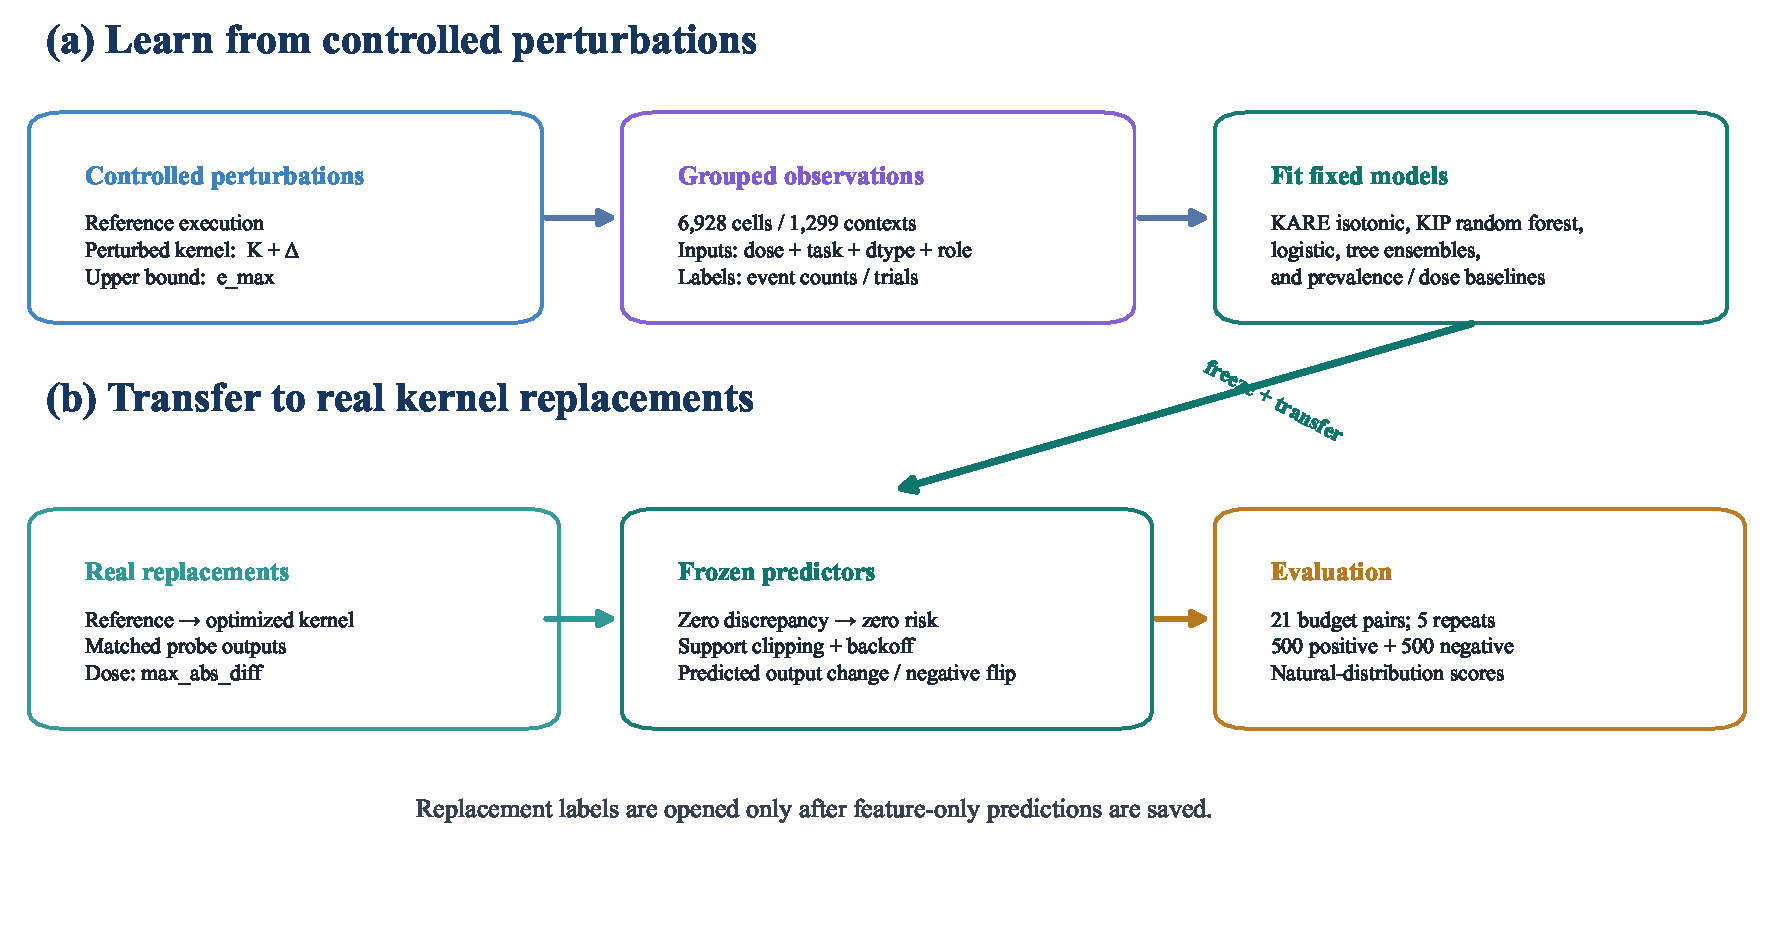
\includegraphics[width=\linewidth]{figures/method-overview.pdf}
  \caption{Paper-aligned workflow. Models are fit on grouped controlled-perturbation observations, frozen, and transferred to real replacements using the measured maximum discrepancy. Replacement labels are opened only after feature-only predictions have been saved.}
  \label{fig:method-overview}
\end{figure}

\subsection{Task and grouped observations}
\label{sec:task}

Let $f_{\mathrm{ref}}(x)$ be the final output of a reference model execution on request $x$, and let $f_{\mathrm{alt}}(x)$ be the output after perturbing or replacing one kernel. Let $C(o,y)\in\{0,1\}$ indicate correctness against the task target $y$. We define
\begin{equation}
 Z_{\mathrm{change}}=\mathbf{1}\{f_{\mathrm{alt}}(x)\neq f_{\mathrm{ref}}(x)\},\qquad
 Z_{\mathrm{flip}}=\mathbf{1}\{C(f_{\mathrm{ref}}(x),y)=1\land C(f_{\mathrm{alt}}(x),y)=0\}.
 \label{eq:events}
\end{equation}
The output comparison uses the task's discrete result: top-1 label for classification, selected answer for multiple-choice QA, parsed answer for GSM8K, extracted span for extractive QA, and decoded transcript for ASR. Negative flip uses the reference-correct-to-alternative-wrong transition.

The perturbation corpus is represented as grouped-binomial observations. A cell is identified by model, logical kernel, dtype, benchmark, and perturbation setting. For endpoint $e$, cell $i$ contains $k_{i,e}$ events among $n_i$ requests, with empirical rate $r_{i,e}=k_{i,e}/n_i$. We retain event and trial counts rather than expanding rates into pseudo-independent rows. The training snapshot has 6,928 cells and 1,299 complete contexts spanning 13 models, seven task scopes, and FP32, FP16, and BF16.

\subsection{Inputs and discrepancy mapping}

The main predictor uses four inputs: $\log_{10}(d)$, task scope, dtype, and the paper's 13-level operator role. The role taxonomy separates attention linear, attention arithmetic, attention PV, attention softmax, normalization, activation, convolution, pooling, MLP projection, generic projection, output head, logit scale, and residual scale. Model identity, candidate identity, and benchmark identity remain available for grouping and diagnostics but are not predictor features.

For a perturbation cell, $d$ is the upper endpoint of its applied magnitude range, denoted \texttt{range\_high}. For a real replacement, we use the maximum absolute difference between matched reference and optimized kernel outputs, denoted \texttt{max\_abs\_diff}. This is a max-to-max mapping that preserves the interpretation of the paper's upper-bound dose. An exact-zero replacement discrepancy receives predicted risk zero. A nonzero value outside role-specific support is evaluated at the nearest supported boundary, with fallback from task--dtype--role to task scope and then to pooled training support.

\subsection{Compared estimators}

We compare eleven alternatives with fixed settings. The prevalence baseline predicts request-weighted training prevalence. Dose-only isotonic regression uses weighted pooled adjacent violators and smoothed rate $(s+0.5)/(n+1)$. Ridge regression uses $\alpha=1$. The multinomial softmax logistic model uses a spline basis of log-dose with task, dtype, and role interactions. RBF support-vector regression uses $C=1$ and $\epsilon=0.02$. The nearest-neighbor estimator averages the 25 closest cosine-distance observations, weighted by trial count and inverse distance. The grouped MLP has two hidden layers (64 and 32 units) and minimizes trial-weighted grouped categorical cross-entropy for the nested outcomes. A single decision tree is restricted to depth 2. ExtraTrees uses 120 randomized trees, depth 8, and leaf size 6. Histogram gradient boosting uses 180 iterations and at most 15 leaves. CatBoost uses CPU MultiRMSE with 220 iterations, depth 4, learning rate 0.05, and L2 regularization 5.

Our primary \kip~random forest uses 120 trees, maximum depth 8, minimum leaf size 6, all available features at each split, and fixed seed 20260905. It jointly regresses the two observed rates in a multi-output model, scaling the negative-flip target by two during fitting and restoring its original scale at prediction. The shared post-fit projection enforces $p_{\mathrm{flip}}\leq p_{\mathrm{change}}$.

All learned predictions are clipped to $[0,1]$ and projected to satisfy $p_{\mathrm{flip}}\leq p_{\mathrm{change}}$. To apply one consistent transfer policy, each context is evaluated on a 61-point geometric dose grid. We replace raw predictions by their nondecreasing upper envelope and use an upper-step lookup for the observed replacement discrepancy. This post-fit policy makes the monotonicity and support behavior explicit for every estimator.

\subsection{Locked replacement evaluation}

The replacement pool contains 2,739 unique records from the current packaged snapshot. We fit each estimator on all perturbation cells, save feature-only replacement predictions, and then open the replacement event counts for scoring. For each budget pair, a model flags a record when either predicted endpoint rate exceeds its corresponding budget. The observed joint-positive label is defined analogously from the two measured rates. The primary score uses 21 pairs drawn from budgets of $0.1\%$, $0.2\%$, $0.5\%$, $1\%$, $2\%$, and $5\%$, retaining pairs where the negative-flip budget is no larger than the output-change budget.

For every pair, we sample 500 positive and 500 negative records with replacement. Within each class and net-accuracy-drop severity band, contexts receive equal total weight. The severity bands are at most $0.5\%$, above $0.5\%$ through $1\%$, and above $1\%$. Accuracy drop is the net correct-to-wrong count after subtracting wrong-to-correct transitions. We repeat each pair five times and reuse the draw manifest across all models, for 105,000 draw positions. The reported F1 values average across budget pairs and repeats. Their uncertainty summary is the mean of the 21 within-budget sample standard deviations across five repeats. Because draws overlap and are sampled with replacement, it describes resampling variability rather than independent-record uncertainty. Balanced scores measure screening discrimination and do not estimate natural replacement prevalence. We inherit master seed 9 from the reference protocol; the source study reports selecting it retrospectively from 128 candidates~\citep{kernel_correctness_protocol}. Our run does not search over seeds, so the five-repeat standard deviations do not include uncertainty from that earlier seed selection.

\section{Experiments}
\label{sec:experiments}

\subsection{Experimental setup}

The run uses the current normalized project snapshot and no new GPU execution. The perturbation input contains 6,928 cells and 1,299 contexts. The replacement feature table contains 2,739 records and the same 1,299 context identities. The implementation uses NumPy 2.1.3, pandas 2.2.3, and scikit-learn 1.6.1. Tree and CatBoost models run on CPU. Every model uses the same role mapping, dose mapping, support policy, and balanced draw manifest. Replacement labels are an external evaluation input rather than a source of model selection.

\subsection{Main comparison}

Table~\ref{tab:balanced} reports the mean over the 21 budget pairs and five fixed repetitions. Joint recall is recall for the union positive class defined by the two budget limits. The two accuracy-drop columns measure recall on records whose net accuracy drop exceeds $0.5\%$ and $1\%$, respectively. Accepted violation fraction is the fraction of records predicted safe that are nevertheless positive under the joint budget label.

\begin{table}[t]
\centering
\caption{Balanced replacement screening. F1 is the mean across 21 budget pairs and five repeats, followed by the mean within-budget sample SD. All reported results use the balanced test draws. KIP random forest is the primary method.}
\label{tab:balanced}
\resizebox{\linewidth}{!}{%
\begin{tabular}{lrrrrrr}
\toprule
Method & F1 $\uparrow$ (mean $\pm$ SD) & Precision $\uparrow$ & Joint recall $\uparrow$ & $>0.5\%$ recall $\uparrow$ & $>1\%$ recall $\uparrow$ & Violation $\downarrow$ \\
\midrule
Prevalence & 0.4867 $\pm$ 0.0066 & 0.4097 & 0.6000 & 0.6388 & 0.6497 & 0.2879 \\
Dose-only isotonic & 0.7468 $\pm$ 0.0104 & 0.6712 & 0.8473 & 0.8521 & 0.8480 & 0.2118 \\
Ridge regression & 0.8075 $\pm$ 0.0113 & 0.7490 & 0.8801 & 0.8154 & 0.7105 & 0.1445 \\
Softmax spline logistic & 0.8338 $\pm$ 0.0116 & 0.7954 & 0.8784 & 0.8239 & 0.7267 & \textbf{0.1353} \\
RBF support-vector regression & 0.8020 $\pm$ 0.0103 & 0.7386 & 0.8827 & 0.8411 & 0.7624 & 0.1444 \\
Weighted k-nearest neighbors & \textbf{0.8484} $\pm$ 0.0112 & \textbf{0.8311} & 0.8678 & 0.8042 & 0.6951 & 0.1373 \\
Grouped MLP & 0.8460 $\pm$ 0.0108 & 0.8261 & 0.8686 & 0.7977 & 0.6770 & 0.1381 \\
Decision tree (depth 2) & 0.7897 $\pm$ 0.0119 & 0.7860 & 0.8168 & \textbf{0.8506} & \textbf{0.7905} & 0.1886 \\
\kip~random forest (primary) & 0.8411 $\pm$ 0.0115 & 0.8220 & 0.8634 & 0.8375 & 0.7638 & 0.1419 \\
ExtraTrees & 0.8384 $\pm$ 0.0113 & 0.8164 & 0.8638 & 0.8274 & 0.7453 & 0.1429 \\
HistGradientBoosting & 0.8384 $\pm$ 0.0117 & 0.8098 & 0.8710 & 0.8302 & 0.7433 & 0.1385 \\
CatBoost & 0.8346 $\pm$ 0.0119 & 0.8017 & \textbf{0.8727} & 0.8409 & 0.7626 & 0.1392 \\
\bottomrule
\end{tabular}}
\end{table}

Weighted k-nearest neighbors has the highest mean F1 (0.8484), followed by the grouped MLP (0.8460) and KIP RF (0.8411). These gaps are small relative to mean within-budget resampling standard deviations of 0.0108--0.0115, so they do not establish a decisive winner. The result still supports KIP RF as a strong, paper-grounded primary model. The shallow tree and RBF-SVR show that strong recall on severe accuracy-drop records can coexist with lower overall F1.

The alternatives expose different screening trade-offs. Softmax logistic has the lowest accepted violation fraction (0.1353), while the depth-2 tree has the highest recall in the >0.5% and >1% net-accuracy-drop subgroups. KNN and MLP perform well in mean F1 but do not dominate every subgroup. Shared draws and fixed settings make this a descriptive comparison, not post-hoc model selection on replacement outcomes.

\begin{figure}[t]
  \centering
  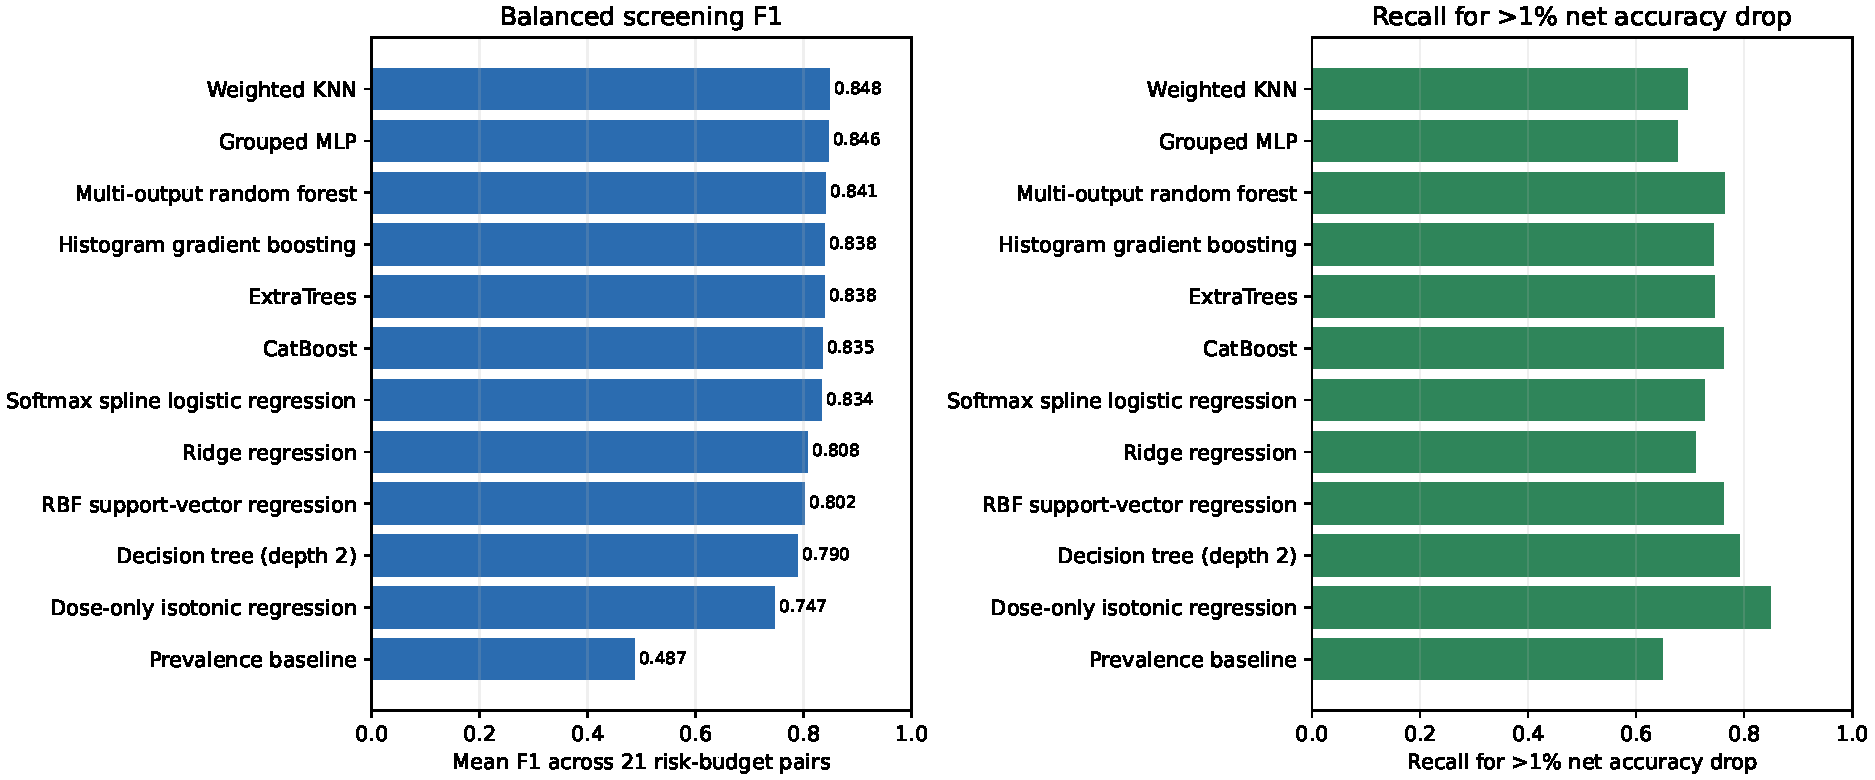
\includegraphics[width=\linewidth]{figures/model-comparison.pdf}
  \caption{Balanced screening F1 and recall for >1\% net-accuracy-drop records across all twelve fixed estimators. Both panels use the same paper-protocol balanced test draws.}
  \label{fig:model-comparison}
\end{figure}

\subsection{Interpretation within the balanced test set}

The formal test set intentionally gives equal positive and negative class counts for each budget pair. Therefore, F1 and precision describe a balanced screening task and should not be read as natural production prevalence or as a calibrated deployment probability. Within that fixed evaluation target, KNN and MLP lead mean F1, KIP RF remains close, and the shallow tree is more conservative on the severe accuracy-drop subgroups. The same draw manifest makes these comparisons paired across methods.

\subsection{Budget sensitivity and applicability}

Figure~\ref{fig:budget-sensitivity} shows F1 over all 21 budget pairs for each method. KIP RF, KNN, MLP, CatBoost, ExtraTrees, and boosting remain comparatively strong, while prevalence, dose-only, and the shallow tree trail in mean F1. Predictions remain frozen throughout this sweep. No estimator is refit or recalibrated for individual budget pairs.

The transfer policy assigns 758 records to the exact-zero state, 1,308 records within role-specific dose support, 110 below support, and 563 above support. Every record receives a numeric prediction for balanced scoring, but its support status is retained. The 673 below- or above-support records therefore carry weaker dose support than in-range records.

\begin{figure}[t]
  \centering
  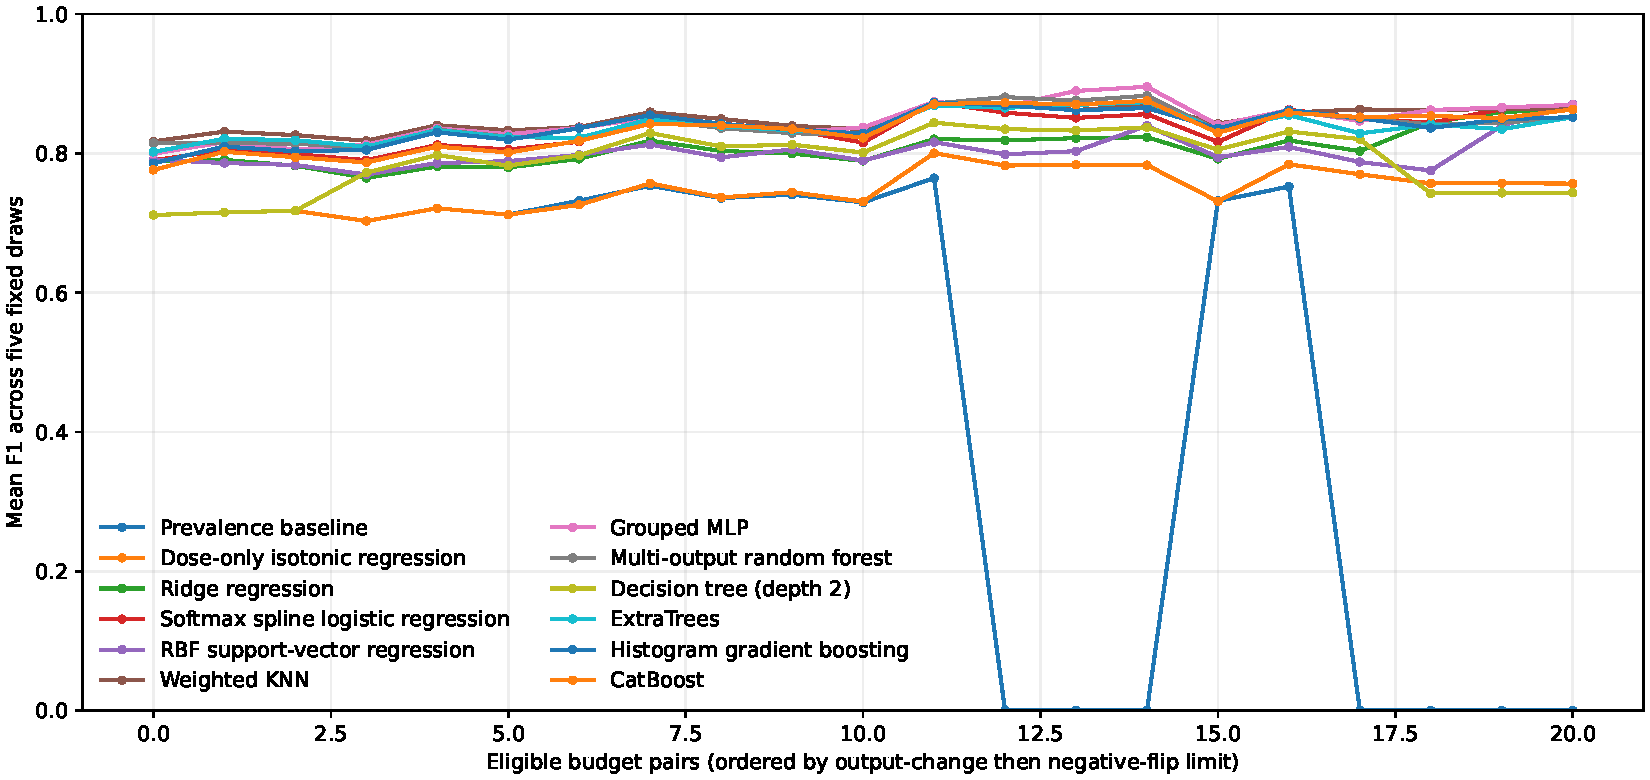
\includegraphics[width=\linewidth]{figures/budget-sensitivity.pdf}
  \caption{Sensitivity of mean balanced F1 to the 21 output-change/negative-flip budget pairs. Predictions remain frozen while the joint positive label changes with the budgets.}
  \label{fig:budget-sensitivity}
\end{figure}

\subsection{Limitations}

The study measures transfer within one packaged data snapshot, 13 models, seven task scopes, and 2,739 replacement records. The perturbation and replacement tables share 1,299 context identities. This evaluation therefore tests transfer across discrepancy-generating mechanisms within covered contexts and does not establish generalization to unseen models or contexts. Maximum absolute discrepancy also discards the sign, distribution, correlation, and accumulation pattern of errors across invocations. Upper-tail labels are sparse, and sampling with replacement can repeatedly select the same high-risk records. Support clipping defines predictions outside the fitted range but does not guarantee calibration for unseen discrepancies. The replacement labels come from the current packaged snapshot and are not identical to every historical validation snapshot reported in the source study.

\section{Conclusion}

We evaluated KIP random forest as the primary method against eleven alternatives using the same balanced external test draws. KIP RF achieved mean F1 of 0.8411 and reproduced the reference RF-C-Max metrics within $5.1\times10^{-7}$. Weighted KNN and MLP were slightly higher, but their differences are small relative to resampling variation. This broad comparison shows that distinct statistical, kernel, neighbor, neural, and ensemble approaches can perform competitively on this task. The predictions remain limited to contexts and discrepancy support represented in the current snapshot.

\section*{Acknowledgments and AI-use disclosure}
OpenAI Codex assisted with analysis-code development and manuscript editing~\citep{openai_codex}. The authors are responsible for the submitted report.

{\small
\bibliographystyle{unsrtnat}
\bibliography{references}
}

\end{document}
